\section{磁场对电流的作用}\label{sec:10-9}

电流能产生磁场,那么,磁场对电流会不会有作用呢?
把一根直导体 $AB$ 放在一个蹄形磁铁的磁场里(图 \ref{fig:10-39}),给导体 $AB$ 通电流的时候,
导体 $AB$ 就运动起来,这说明\CJKunderwave{通电导体在磁场里要受到力的作用}。

\begin{figure}[htbp]
    \centering
    \begin{minipage}{10cm}
    \centering
    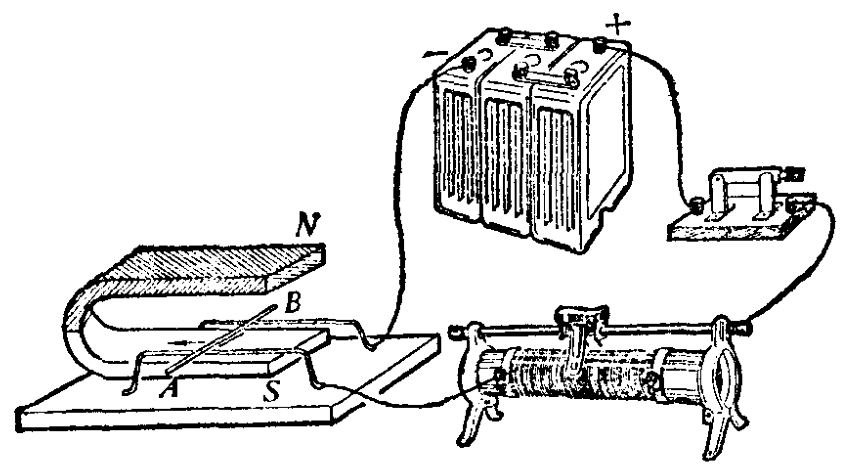
\includegraphics[width=10cm]{../pic/czwl2-ch10-39}
    \caption{}\label{fig:10-39}
    \end{minipage}
    \qquad
    \begin{minipage}{5cm}
    \centering
    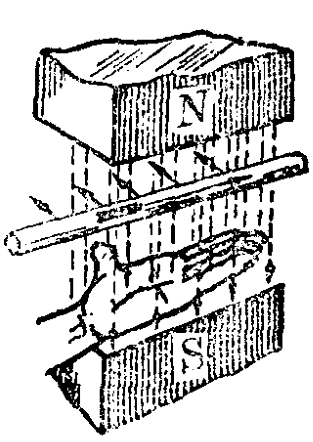
\includegraphics[width=4cm]{../pic/czwl2-ch10-40}
    \caption{}\label{fig:10-40}
    \end{minipage}
\end{figure}


在图 \ref{fig:10-39} 所示的实验中,如果改变电流的方向,导体运动的方向就随着改变;
如果改变磁力线的方向,导体运动的方向也随着改变。
这表明通电导体在磁场里受到的力的方向跟磁力线的方向和电流的方向都有关系。

通电导体受力的方向和磁力线方向、电流方向之间的关系,可以用左手定则来判定:
伸开左手,使大拇指跟其余四个手指垂直,并且都跟手掌在一个平面内。
把左手放入磁场中,让磁力线垂直穿入手心,并使伸开的四指指向电流的方向,
那么,拇指所指的方向,就是通电导体在磁场中的受力方向(图 \ref{fig:10-40})。

如果把一个通电线圈放在磁场里,它将怎样运动呢?

\begin{figure}[htbp]
    \centering
    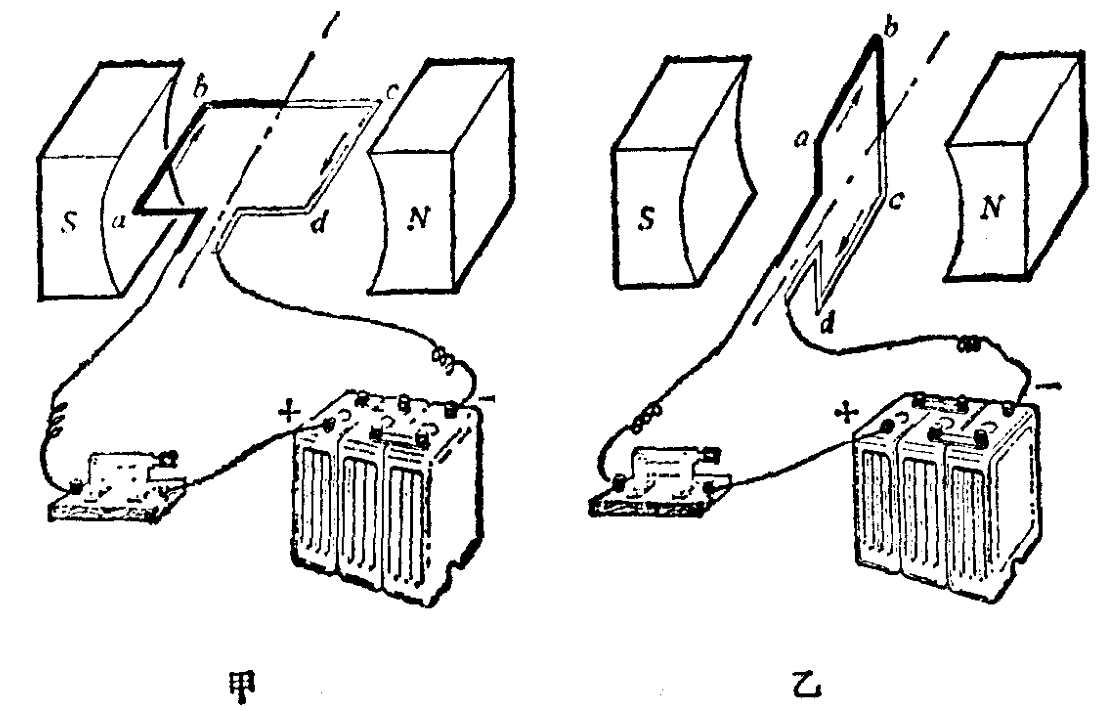
\includegraphics[width=0.7\textwidth]{../pic/czwl2-ch10-41}
    \caption{}\label{fig:10-41}
\end{figure}

照图 \ref{fig:10-41} 甲那样,把一个矩形线圈放在磁场里,我们会看到,
当线圈中通过电流时,线圈发生转动,但线圈并不能持续地转动下去,
而是转到图 \ref{fig:10-41} 乙的位置便停了下来。
线圈为什么会转动,又为什么不能继续转动下去呢?
根据左手定则可以知道,在图甲的位置时,$ab$ 边受到一个向上的力,$cd$ 边受到一个向下的力,
因而线圈沿着顺时针方向转动起来。
当线圈平面转到跟磁力线方向垂直的时候(图 \ref{fig:10-41} 乙),$ab$ 边和 $cd$ 边受到的力恰好在同一直线上,
而且大小相等,方向相反,所以线圈就停在这个平衡位置上。


如果开始实验的时候,线圈中的电流方向跟上面实验里的相反,线圈就要向相反的方向转动。
想想看,为什么会这样?

通电导体和通电线圈在磁场里受到力的作用而发生运动的时候,消耗了电能,得到了机械能。
在这种现象里\CJKunderwave{电能转化为机械能}。

